\section{Grenzwerte und Konvergenz}

\subsection{Grenzwerte von Funktionen}

\begin{definition}{Konvergenz einer Funktion}\\
    Die Funktion $y = f(x)$ hat an der Stelle $x_0$ den Grenzwert $y_0$ falls:\\
    für jede Folge $\left(x_{n}\right)$ mit $\lim _{n \rightarrow \infty} x_{n}=x_{0}$ gilt $\lim _{n \rightarrow \infty} f\left(x_{n}\right)=y_{0}$\\
    Bmk: Die Stelle $x_{0}$ muss nicht im Definitionsbereich $D$ sein.
\end{definition}

\begin{concept}{Konvergenz/Divergenz}
    \begin{itemize}
        \item Konvergenz:
        Funktion mit Grenzwert $x \rightarrow \infty$
        \item Divergenz:
        Funktion ohne Grenzwert $x \rightarrow \infty$
        \item Bestimmte Divergenz:
        Funktion mit $\lim _{x \rightarrow \infty} f(x)= \pm \infty$
    \end{itemize}
\end{concept}

\begin{theorem}{Rechnen mit Grenzwerten von Funktionen}
    \begin{itemize}
        \item $\lim_{x \to x_0} (f + g)(x) = \lim_{x \to x_0} f(x) + \lim_{x \to x_0} g(x)$
        \item $\lim_{x \to x_0} (f \cdot g)(x) = \lim_{x \to x_0} f(x) \cdot \lim_{x \to x_0} g(x)$
        \item Sei $f \leq g$, so ist $\lim_{x \to x_0} f(x) \leq \lim_{x \to x_0} g(x)$
        \item Falls $g_1 \leq f \leq g_2$ und $\lim_{x \to x_0} g_1(x) = \lim_{x \to x_0} g_2(x)$, so existiert $\lim_{x \to x_0} f(x) = \lim_{x \to x_0} g_1(x)$
    \end{itemize}
\end{theorem}

\begin{highlight}{Wichtige Grenzwerte}
    \begin{center}
        \begin{minipage}{0.45\linewidth}
            \tcbsubtitle{Harmonische Folge:}
            $$\lim _{n \rightarrow \infty} \frac{1}{n}=0$$
            \tcbsubtitle{Geometrische Folge:}
            $$\lim _{n \rightarrow \infty} q^n=0 \quad(q<1)$$
        \end{minipage}
        \hfill\vline\hfill
        \begin{minipage}{0.45\linewidth}
            \tcbsubtitle{n-te Wurzel:}
            $$\lim _{n \rightarrow \infty} \sqrt[n]{a}=1$$
            \tcbsubtitle{Eulerzahl:}
            $$\lim _{n \rightarrow \infty}\left(1+\frac{1}{n}\right)^n=e$$
        \end{minipage}
    \end{center}
\end{highlight}

\begin{formula}{Spezielle Grenzwerte}

    \textcolor{pink}{$n\rightarrow \infty$}

    %resize contents to linewidth for very wide tables or formulas
    \resizebox*{\linewidth}{!}{
    \begin{tabular}{c|c|c|c}
        \(\frac{1}{n}\rightarrow 0\) & \(e^n\rightarrow \infty\) & \(\frac{1}{n^k}\rightarrow 0\ \ \forall k\in \mathbb{R}^+\) & \(\frac{\log{n}}{n-1}\rightarrow 1\)\\
        \hline
        \(c+\frac{1}{n}\rightarrow c\) & \(e^{-n}\rightarrow 0\) & \((1+n)^{\frac{1}{n}}\rightarrow 1\) & \(\frac{n^n}{n!}\rightarrow \infty\)\\
        \hline
        \(\frac{c\cdot n}{c^n}\rightarrow 0\) & \(\frac{e^n}{n^c}\rightarrow \infty\) & \(\left(1+\frac{1}{n}\right)^c \rightarrow 1\) & \(\left(\frac{n}{n+c}\right)^n\rightarrow e^{-c}\)\\
        \hline
        \(\sqrt[n]{n}=n^{\frac{1}{n}}\rightarrow 1\) & \(\frac{\sin{n}}{n}\rightarrow 0\) & \(\left(1+\frac{1}{n}\right)^n \rightarrow e\) & \(\frac{\ln{n}}{n}\rightarrow 0\)\\
        \hline
        \(\sqrt[n]{n!}\rightarrow \infty\) & \(\arctan{n}\rightarrow \frac{\pi}{2}\) & \(\left(1+\frac{c}{n}\right)^n \rightarrow e^c\) & \(\frac{c^n}{n!} \rightarrow 0\)\\
        \hline
        \(\frac{1}{n}\sqrt[n]{n!} \rightarrow \frac{1}{e}\) & \(\ln{n}\rightarrow \infty\) & \(\left(1-\frac{1}{n} \right)^n \rightarrow \frac{1}{e}\) & 
    \end{tabular}
    }

    $$n^c\cdot q^n \rightarrow 0 \quad \forall c \in \mathbb{Z},0\leq q \leq 1$$
    $$n(\sqrt[n]{c}-1)\rightarrow \ln{c}\quad \forall c > 0$$

    \textcolor{pink}{$n\rightarrow 0$}

    %or size up tables with complex formulas for better readability
    \resizebox*{0.7\linewidth}{!}{
    \begin{tabular}{c|c|c}
        \(\ln{n}\rightarrow -\infty\)&\(\frac{\sin{n}}{n}\rightarrow 1\)&\(\frac{1}{\arctan{n}}\rightarrow 1\)\\
        \hline
        \(n\log{n}\rightarrow 0\)&\(\frac{\cos{(n)}-1}{n}\rightarrow 0\)&\(\frac{e^n-1}{n}\rightarrow 1\)\\
        \hline
        \(\frac{\log{1}-n}{n}\rightarrow -1\)&\(\frac{1}{\cos{n}}\rightarrow1\)&\(\frac{e^cn-1}{n}\rightarrow c\)\\
        \hline 
        \(\frac{c^n-1}{n}\rightarrow\ln{c},\forall c>0\)&\(\frac{1-\cos{n}}{n^2}\rightarrow
        \frac{1}{2}\)&\((1+n)^{\frac{1}{n}}\rightarrow e\)\\
    \end{tabular}
    }
\end{formula}

\begin{KR}{Grenzwert Berechnen Tricks}
    \begin{itemize}
        \item " $\frac{\infty}{\infty} "$ Trick: Erweitern mit $\frac{1}{n^{k}}$ (k: grösster Exponent)
    \end{itemize}
    
    $\lim _{n \rightarrow \infty} \frac{2 n^{6}-n^{3}}{7 n^{6}+n^{5}-3} \cdot \frac{\frac{1}{n^{6}}}{\frac{1}{n^{6}}}=\frac{2}{7}$
    
    \begin{itemize}
        \item " $\frac{\infty}{\infty} "$ Trick: Erweitern mit $\frac{1}{a^{k}}$ (a: grösste Basis, k: kleinster Exponent) $\lim _{n \rightarrow \infty} \frac{7^{n-1}+2^{n+1}}{7^{n}+5} \cdot \frac{\frac{1}{7^{n-1}}}{\frac{1}{7^{n-1}}}=\frac{1}{7}$
        \item " $\infty-\infty$ " Trick: Erweitern mit $\sqrt{\cdots}+\sqrt{\cdots}$
    \end{itemize}
    
    $\lim _{n \rightarrow \infty}\left(\sqrt{n^{2}+n}-\sqrt{n^{2}+1}\right)=1 / 2$
    
    \begin{itemize}
        \item e-like...: Trick: umformen zu $\left(\left(1+\frac{1}{x}\right)^{x}\right)^{a} \Rightarrow e^{a}$
    \end{itemize}
\end{KR}

\raggedcolumns
\columnbreak

\subsection{Grenzwerte von Folgen}

\begin{definition}{Formelle Grenzwert Definition}
    Folgende Aussagen sind äquivalent:
    \begin{enumerate}
        \item $\sequence$ konvergiert gegen $l = \lim_{n \to \infty} a_n$
        \item $\forall \varepsilon > 0~\exists N \geq 1$, sodass $|a_n -l | < \varepsilon \quad \forall n \geq N$.
    \end{enumerate}
\end{definition}

\begin{remark}
    Bem: $l$ bezeichnet den Grenzwert $\lim_{n \to \infty} a_n$
\end{remark}

\begin{lemma}{Einzigartigkeit Grenzwert}
    Es gibt max. ein $l \in \R$ für $a_n$ mit dieser Eigenschaft (max. 1 Grenzwert)
\end{lemma}

\begin{theorem}{Rechenregeln mit Folgen}\\
    Sei $\sequence,\sequence[b]$ konvergente Folgen mit$a = \lim_{n \to \infty} a_n$, $b = \lim_{n \to \infty} b_n$
    \begin{enumerate}
        \item $(a_n \pm b_n)_{n \geq 1}$ konvergent, $\lim_{n \to \infty} (a_n \pm b_n) = a \pm b$.
        \item $(a_n \cdot b_n)_{n \geq 1}$ konvergent, $\lim_{n \to \infty} (a_n \cdot b_n) = a \cdot b$.
        \item $(a_n \div  b_n)_{n \geq 1}$ konvergent, $\lim_{n \to \infty} (a_n \div b_n) = a \div b$.
        \\(solange $b_n \neq 0 ~ \forall n \geq 1$ und $b \neq 0$)
        \item Falls $\exists K \geq 1$ mit $a_n \leq b_n ~ \forall n \geq K$ folgt $a \leq b$.
    \end{enumerate}
\end{theorem}

\begin{KR}{Konvergenz Folgen}
    \begin{enumerate}
        \item Für Brüche, grösste Potenz von n ausklammern und kürzen. Alle übrigen Brüche der Form $\frac{a}{n^s}$ streichen, da diese zu 0 konvergieren.
        \item Für Wurzeln in einer Summe, multipliziere mit der Differenz der Summe (bei a + b multipliziere mit a - b)
        \item Anwendung Satz von Weierstrass/Sandwich-Satz 
        \item Vergleich mit Referenz-Folgen (Spezielle Grenzwerte)
        \item Umformen/Tricks
        \item Definition der Konvergenz/Limes anwenden
        \item Suchen eines konvergenten Majoranten
    \end{enumerate}
\end{KR}

\begin{KR}{Divergenz Folgen}
    \begin{enumerate}
        \item  Suche einen divergenten Minoranten
        \item Für alternierende Folgen zeige, dass \\$\lim_{n \to \infty} a_p1(n) \neq \lim_{n \to \infty} a_p2(n)$
    \end{enumerate}
\end{KR}

\begin{concept}{Satz von Weierstrass}
    \begin{itemize}
        \item $\sequence$ monoton wachsend und nach oben beschränkt. $\Rightarrow$ $\sequence$ konvergiert mit $\lim_{n \to \infty} a_n = \sup \{a_n : n \geq 1\}$
        \item $\sequence$ monoton fallend und nach unten beschränkt. $\Rightarrow$ $\sequence$ konvergiert mit $\lim_{n \to \infty} a_n = \inf \{a_n : n \geq 1\}$
    \end{itemize}
\end{concept}

\begin{theorem}{Sandwich-Satz}
    Sei $\lim a_n = \alpha$ und $\lim c_n = \alpha$ und $a_n \leq b_n \leq c_n, \forall n \geq k$ dann gilt $\lim b_n = \alpha$\\
    Bmk: k steht hier für eine beliebige natürliche Zahl, ab der die Bedingung immer gilt. Also wie bei der Grenzwert-Definition mit dem <<Gürtel>> um den Grenzwert - das gilt ja auch erst ab einem gewissen Wert n.\\
    Bmk 2: Einfach gesagt heisst das, dass wenn wir den Grenzwert von zwei Folgen bereits kennen und dieser für beide gleich ist, und wir eine dritte Folge haben die <<zwischen>> die zwei bekannten Folgen passt (daher Sandwich-Satz), wissen wir dass auch die dritte Folge den gleichen Grenzwert wie die anderen zwei hat.
\end{theorem}    

\begin{KR}{Binom Trick}\\
    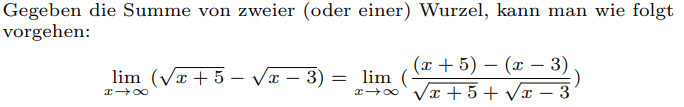
\includegraphics[scale=0.5]{binomtrick.png}
\end{KR}

\begin{KR}{Substitutions Trick}\\
    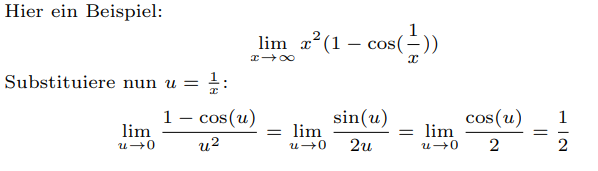
\includegraphics[scale=0.5]{substitutionstrick.png}
\end{KR}

\raggedcolumns
\columnbreak

\subsection{Grenzwerte von Reihen}

\mult{2}

\begin{concept} {Nullfolgenkriterium}\\
    $\sum_{k=1}^\infty a_k~\text{konvergiert} \Rightarrow \lim_{k \to \infty} a_k = 0$ aber die Umkehrung stimmt nicht.
\end{concept}

\begin{concept} {Cauchy Kriterium}\\
    Die Reihe $\sum_{k=1}^\infty a_k$ ist genau dann konvergent, falls:\\
    $\forall \varepsilon > 0 ~\exists N \geq 1$ mit $\left|\sum_{k=n}^m a_k \right| < \varepsilon \quad \forall m \geq n \geq N$
\end{concept}

\begin{concept} {Leibniz Kriterium}\\
    Sei $\sequence$ monoton fallend, mit $a_n \geq 0~\forall n \geq 1$ und $\lim_{n \to \infty} a_n = 0$. Dann konvergiert\\
    $S \coloneqq \sum_{k = 1}^{\infty} (-1)^{k+1} a_k$
    und es gilt: $a_1 - a_2 \leq S \leq a_1$.
\end{concept}

\begin{concept} {Majorantenkriterium}\\
    Seien $a_n, b_n \geq 0$ mit $a_n \geq b_n \quad \forall n > n_0$:\\
    $\sum_{n=0}^\infty a_n$ konvergiert $\Rightarrow \sum_{n=0}^\infty b_n$ konvergiert 
\end{concept}

\begin{concept} {Minorantenkriterium}\\
    Seien $a_n, b_n \geq 0$ mit $a_n \leq b_n \quad \forall n > n_0$:\\
    $\sum_{n=0}^\infty a_n$ divergiert $\Rightarrow \sum_{n=0}^\infty b_n$ divergiert 
\end{concept}

\begin{concept} {Quotientenkriterium}\\
    Sei $\sequence$ mit $a_n \neq 0~\forall n \geq 1$ und: $q = \frac{|a_{n + 1}|}{|a_n|}$\\
    Falls:
    \begin{itemize}
        \item $q < 1$ konvergiert $\sum_{n=1}^\infty a_n$ absolut
        \item $q > 1$ divergiert $\sum_{n=1}^\infty a_n$
    \end{itemize}
    Für $\liminf a_n = 1$ keine Aussage möglich

    \emph{!!! für die harmonische Reihe ist dieses Kriterium nicht anwendbar/gültig !!!}
\end{concept}

\begin{concept} {Wurzelkriterium}\\
    Es sei: $q = \sqrt[n]{|a_n|}$\\
    Dann gilt:
    \begin{itemize}
        \item $q < 1 \Rightarrow \sum_{n=1}^\infty a_n$ konvergiert 
        \item $q > 1 \Rightarrow \sum_{n=1}^\infty a_n$ und $\sum_{n=1}^\infty |a_n|$ divergieren
        \item $q = 1 \Rightarrow$ keine Aussage möglich
    \end{itemize}
\end{concept}

\multend

\begin{KR}{Logarithmus abschätzen}\\
    $\log_b (n)$ kann mit $n^\alpha$ ($\alpha > 0$) abgeschätzt werden.\\
    $\ln(n) \leq \sqrt{n}$
\end{KR} 

\begin{formula}{Reihen - Funktionen}\\
    $
    \begin{array}{ll}
        \sum^{n}_{k=1} k = \frac{n \cdot (n+1)}{2} & \sum^{n}_{k=1} (2k - 1)^2 = \frac{n \cdot (4n^2-1)}{3}\\
        \sum^{n}_{k=1} 2k-1 = n^2 & \sum^{n}_{k=1} k^3 = \left( \frac{n \cdot (n+1)}{2}\right)^2\\
        \sum^{n}_{k=1} 2k = n(n+1) & \sum^{n}_{k=1} \frac{1}{k(k+1)} = \frac{n}{n+1}\\
        \sum^{n}_{k=1} k^2 = \frac{n \cdot (n+1) \cdot (2n+2)}{6} &
    \end{array}
    $
\end{formula}

